\chapter{实验原理与设计}
\section{实验器材与材料}
\subsection{原子力显微镜}
\paragraph*{}
原子力显微镜(Atomic Force Microsocpe,以下简称AFM)是由IBM公司苏黎世研究中心的Gerd Binning于1985年所发明。Binning和他的另一位同事Rohrer于1982年共同发明了世界上首台扫描隧道显微镜(Scanning Tunneling Microscope,以下简称STM),实现原子分辨率的成像,二人也因此获得了1986年的诺贝尔物理学奖。STM是基于样品和扫描探针之间的隧道电流来工作的,因此只能探测导体以及半导体材料的表面形貌;另外,隧穿电流与表面态费米能处的电子态密度有关,因此STM测量得到的实际上是表面形貌和电子态共同作用的结果,并不是样品准确的表面形貌特征。为了弥补STM的不足,Binning于1985年发明了基于原子之间的van der Waals力工作的AFM。如图\ref{fig:7}所示。AFM是通过探针和样品表面原子间的相互作用力来进行成像的,因此不受材料导电性质的影响,同时也具有纳米级的分辨率。
\begin{figure}
	\centering
	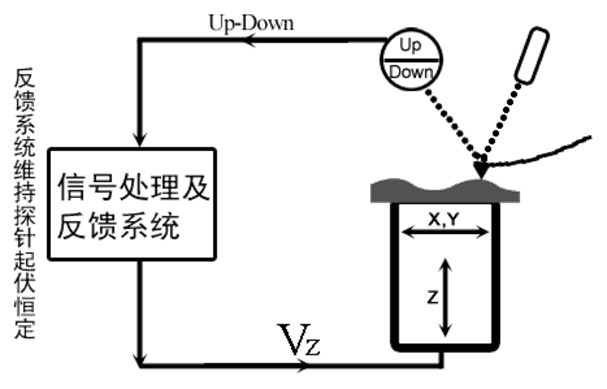
\includegraphics[width=0.7\linewidth]{figures/AFM1}
	\caption{原子力显微镜工作原理示意图}
	\label{fig:7}
\end{figure}
\paragraph*{}
AFM的工作原理很简单。首先将样品放置在扫描器上方,扫描器中的压电陶瓷管在外加电压的作用下,可以在 X、 Y 和 Z 方向上独立运动。AFM探头中的激光器发出激光,照射在悬臂梁背面,经反射后,落在光斑位置检测器(四象限)上。光斑位置检测器上下部分的光强差产生了上下部分的电压差,通过测量这个压差,就可以得到光斑位置的变化量。在接触模式中,探针的针尖部分保持与样品表面接触。当探针在样品表面扫描时,由于样品表面的原子与微悬臂探针尖端的原子间的相互作用力,微悬臂将随样品表面形貌而弯曲起伏,反射光束也将随之偏移,光斑位置检测器上下部分的电压差值也发生改变。反馈电路测量这个差值,通过改变加在扫描器 Z 方向上的电压,保持这个差值的恒定,计算机记录这个电压,即反映了样品的表面形貌。
\paragraph*{}
本文使用的是广州市本原纳米仪器有限公司生产的CSPM5500扫描探针显微镜系统,实物图如图\ref{fig:8}所示。
\begin{figure}
	\centering
	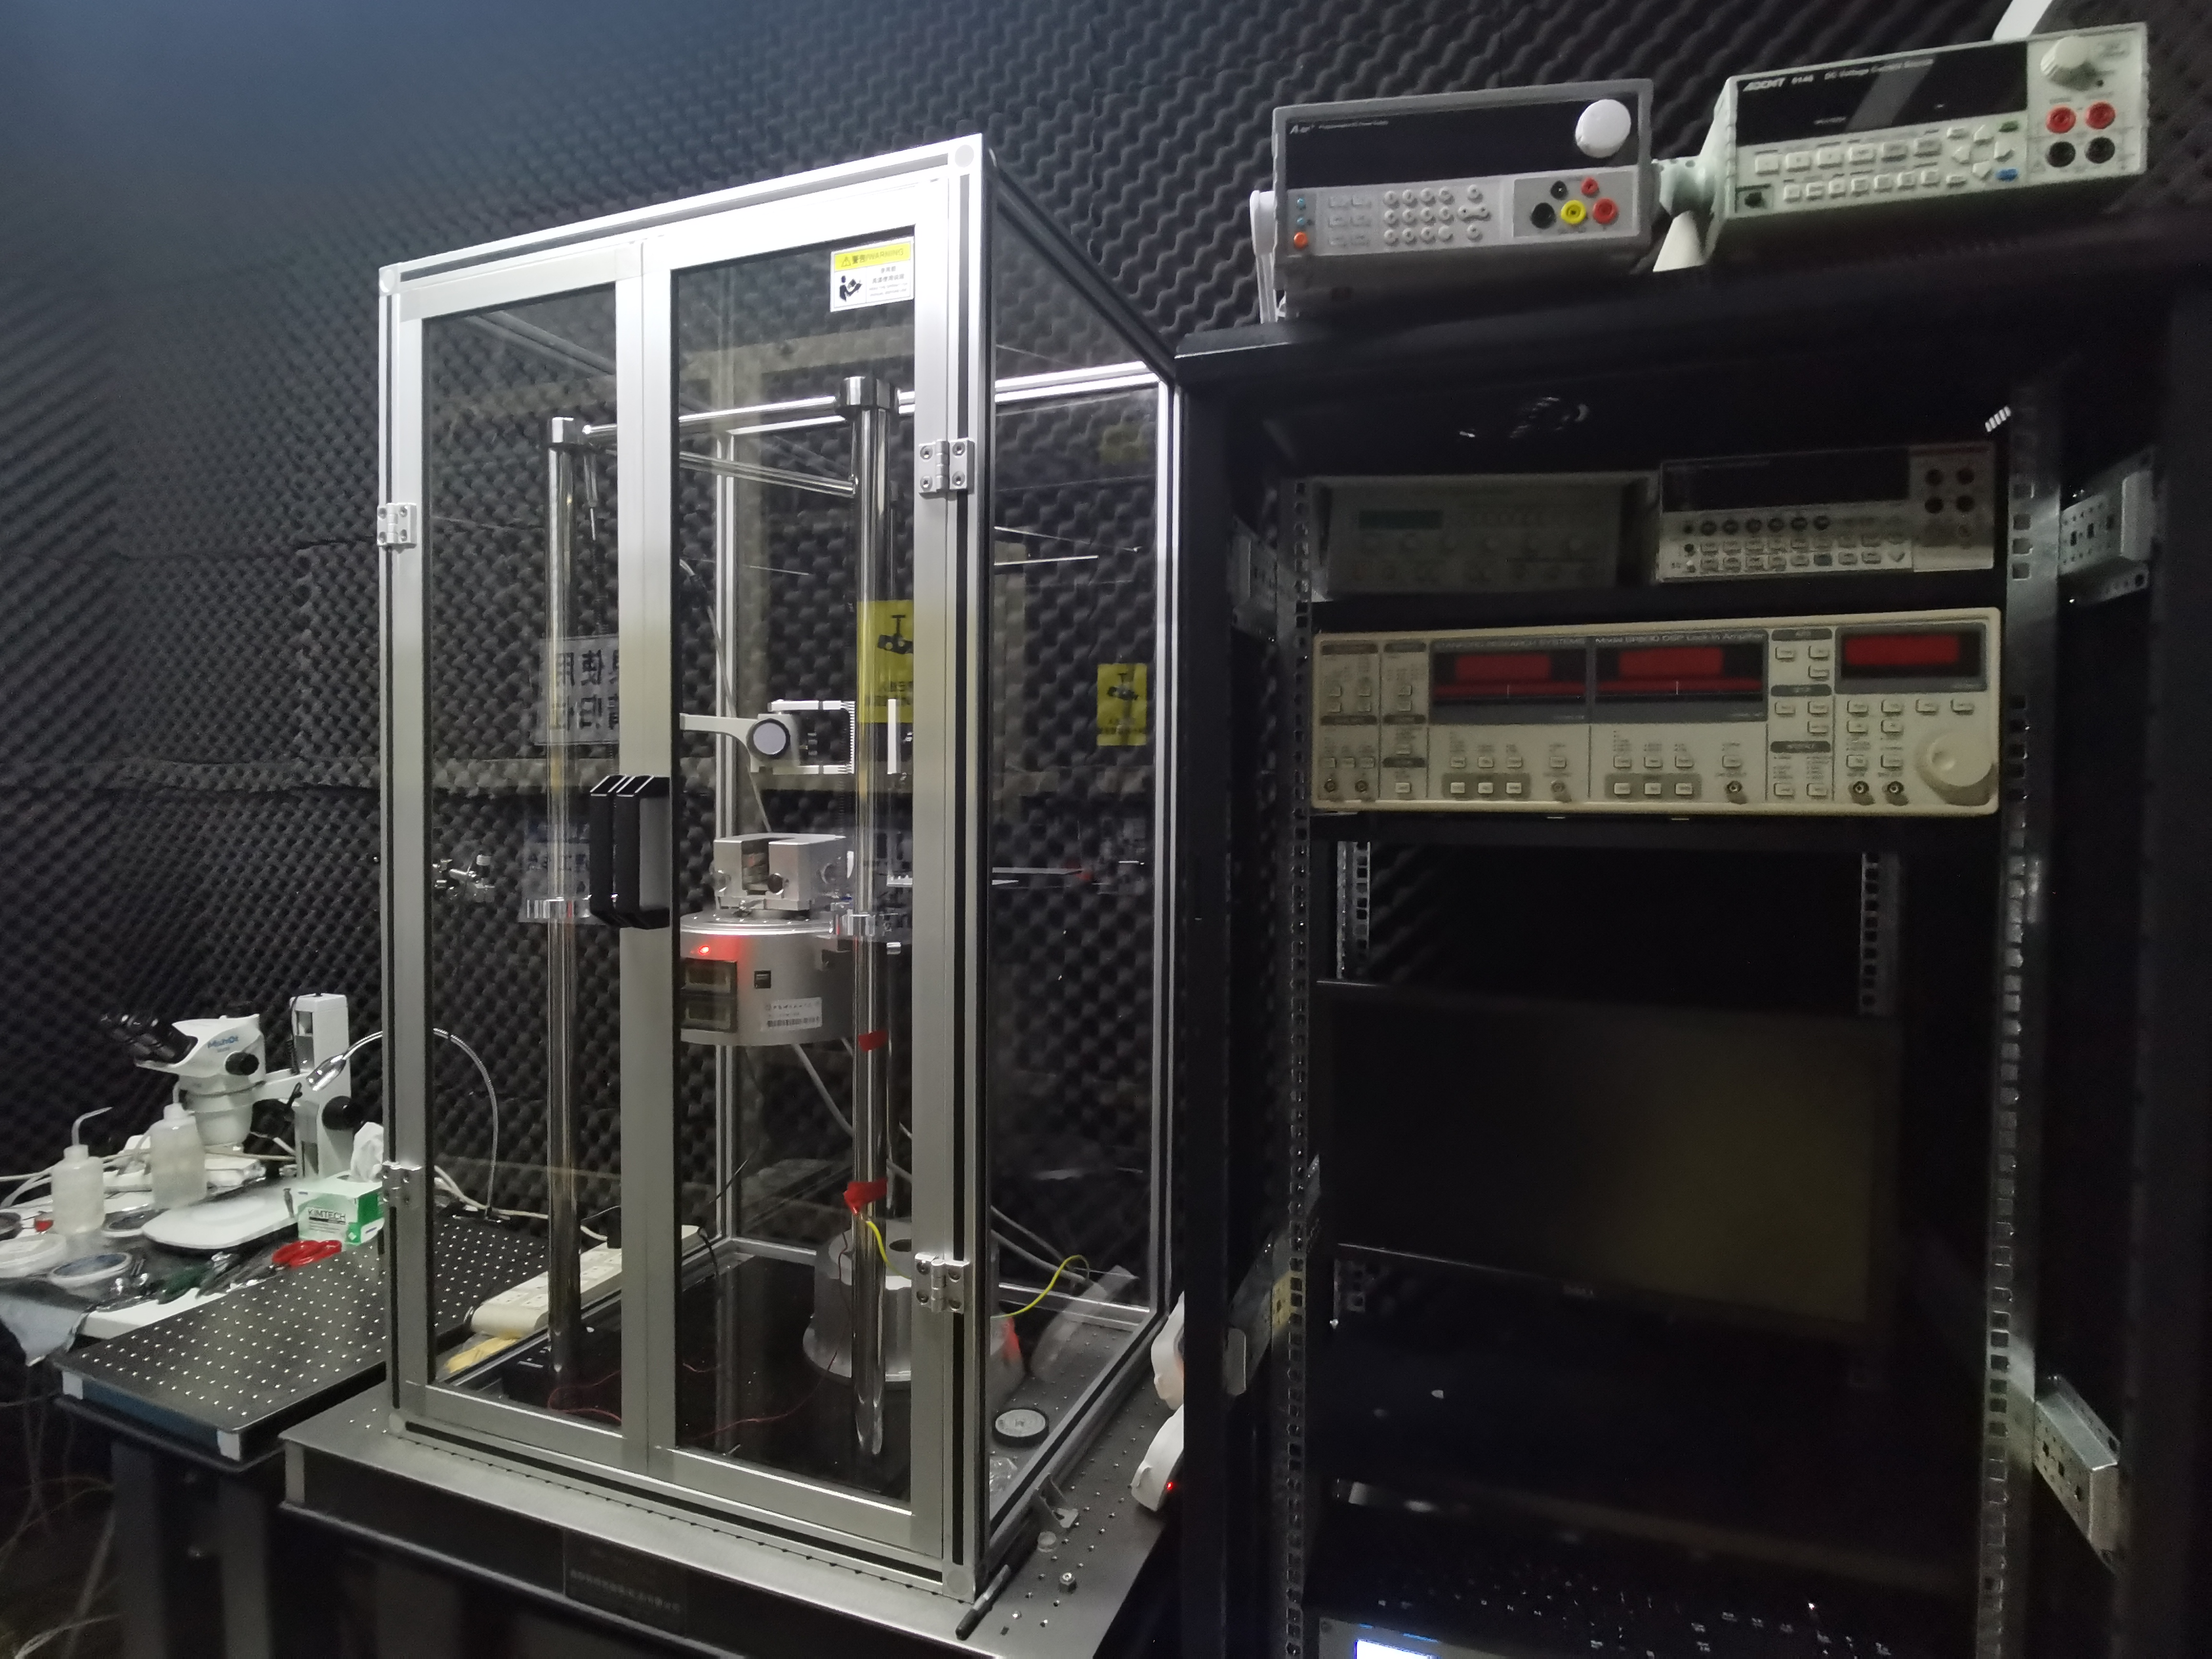
\includegraphics[width=0.7\linewidth]{原子力显微镜实物图}
	\caption{原子力显微镜系统实物图}
	\label{fig:8}
\end{figure}
\subsection{制备探针}
为了测量金球与金板之间的Casimir力,我们需要在悬臂梁下方粘上金球。我们使用的方法是在空悬臂梁下面粘上镀金的聚苯乙烯小球作为实验所用的探针,空悬臂梁采用的是APPNANO公司生产的"HYDRA6V-200NG-TL-50"型号悬臂梁。具体步骤为先使用AB银胶将直径大约为100$\mu$m的聚苯乙烯小球粘到空悬臂梁上,然后使用电子束热蒸发的方法在小球表面先后镀上5nm的Ti和100nm的Au,最后用扫描电子显微镜观察粘上小球的针尖如图\ref{fig:9}所示。
\begin{figure}
	\centering
	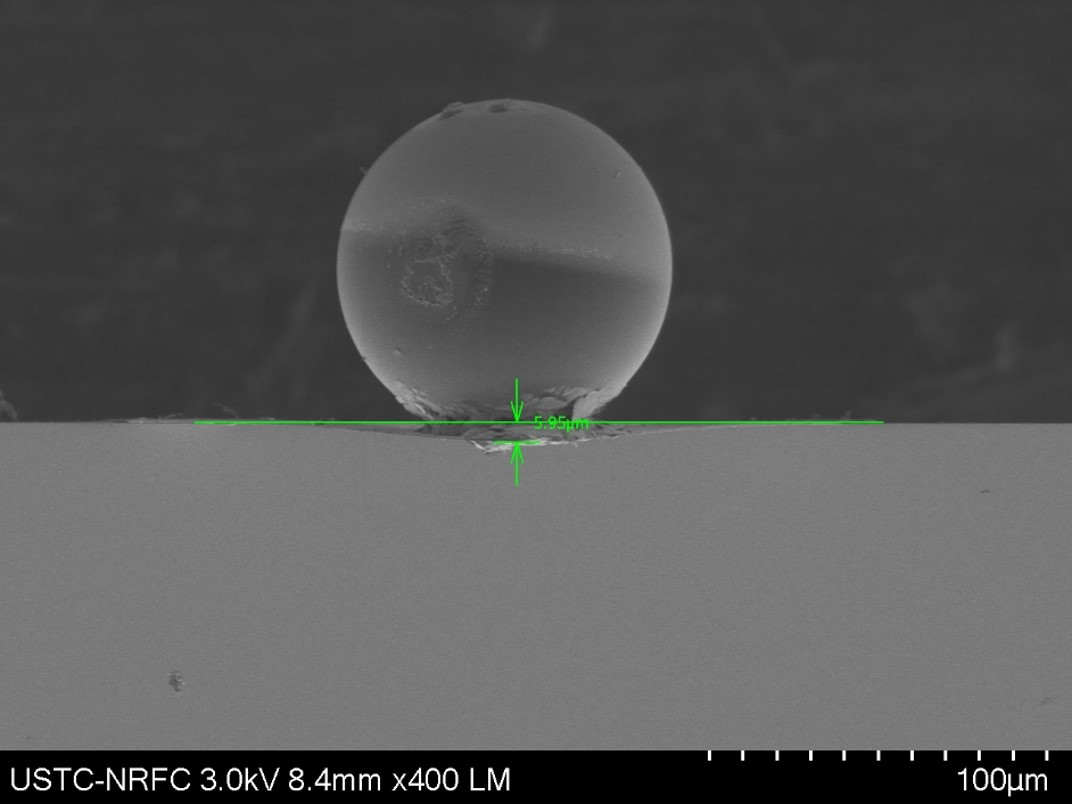
\includegraphics[scale=0.4]{figures/粘小球的针尖}
	\caption{粘上小球的针尖}
	\label{fig:9}
\end{figure}
\newpage
\subsection{制作样品以及接地线}
为了得到表面比较平整的金板,我们使用磁控溅射的方法来制备金样品,镀膜参数为在氧化硅表面先后镀上15nm的Ti和100nm的Au。在实验过程中,静电力会对Casimir力的探测造成很大的干扰。我们分析了可能引起静电力的因素:金样品表面带电和探针表面带电。为了排除静电力对于实验的影响,我们需要在样品上接地线,将样品表面的电荷导出。我们采用的方法是用导电银胶将一根铜线粘在样品表面,在实验过程中将铜线连接至外接的地线以达到样品接地的效果,如图\ref{fig:10}(a)所示。图\ref{fig:10}(b)为接地后测量的样品表面到地线之间的电阻值。利用这种方法可以明显减弱静电力对实验的影响,但是无法完全消除,要想完全消除静电力的干扰,需要使用动态锁频的方法\cite{deMan_2009}。
\begin{figure}[h]
	\centering
	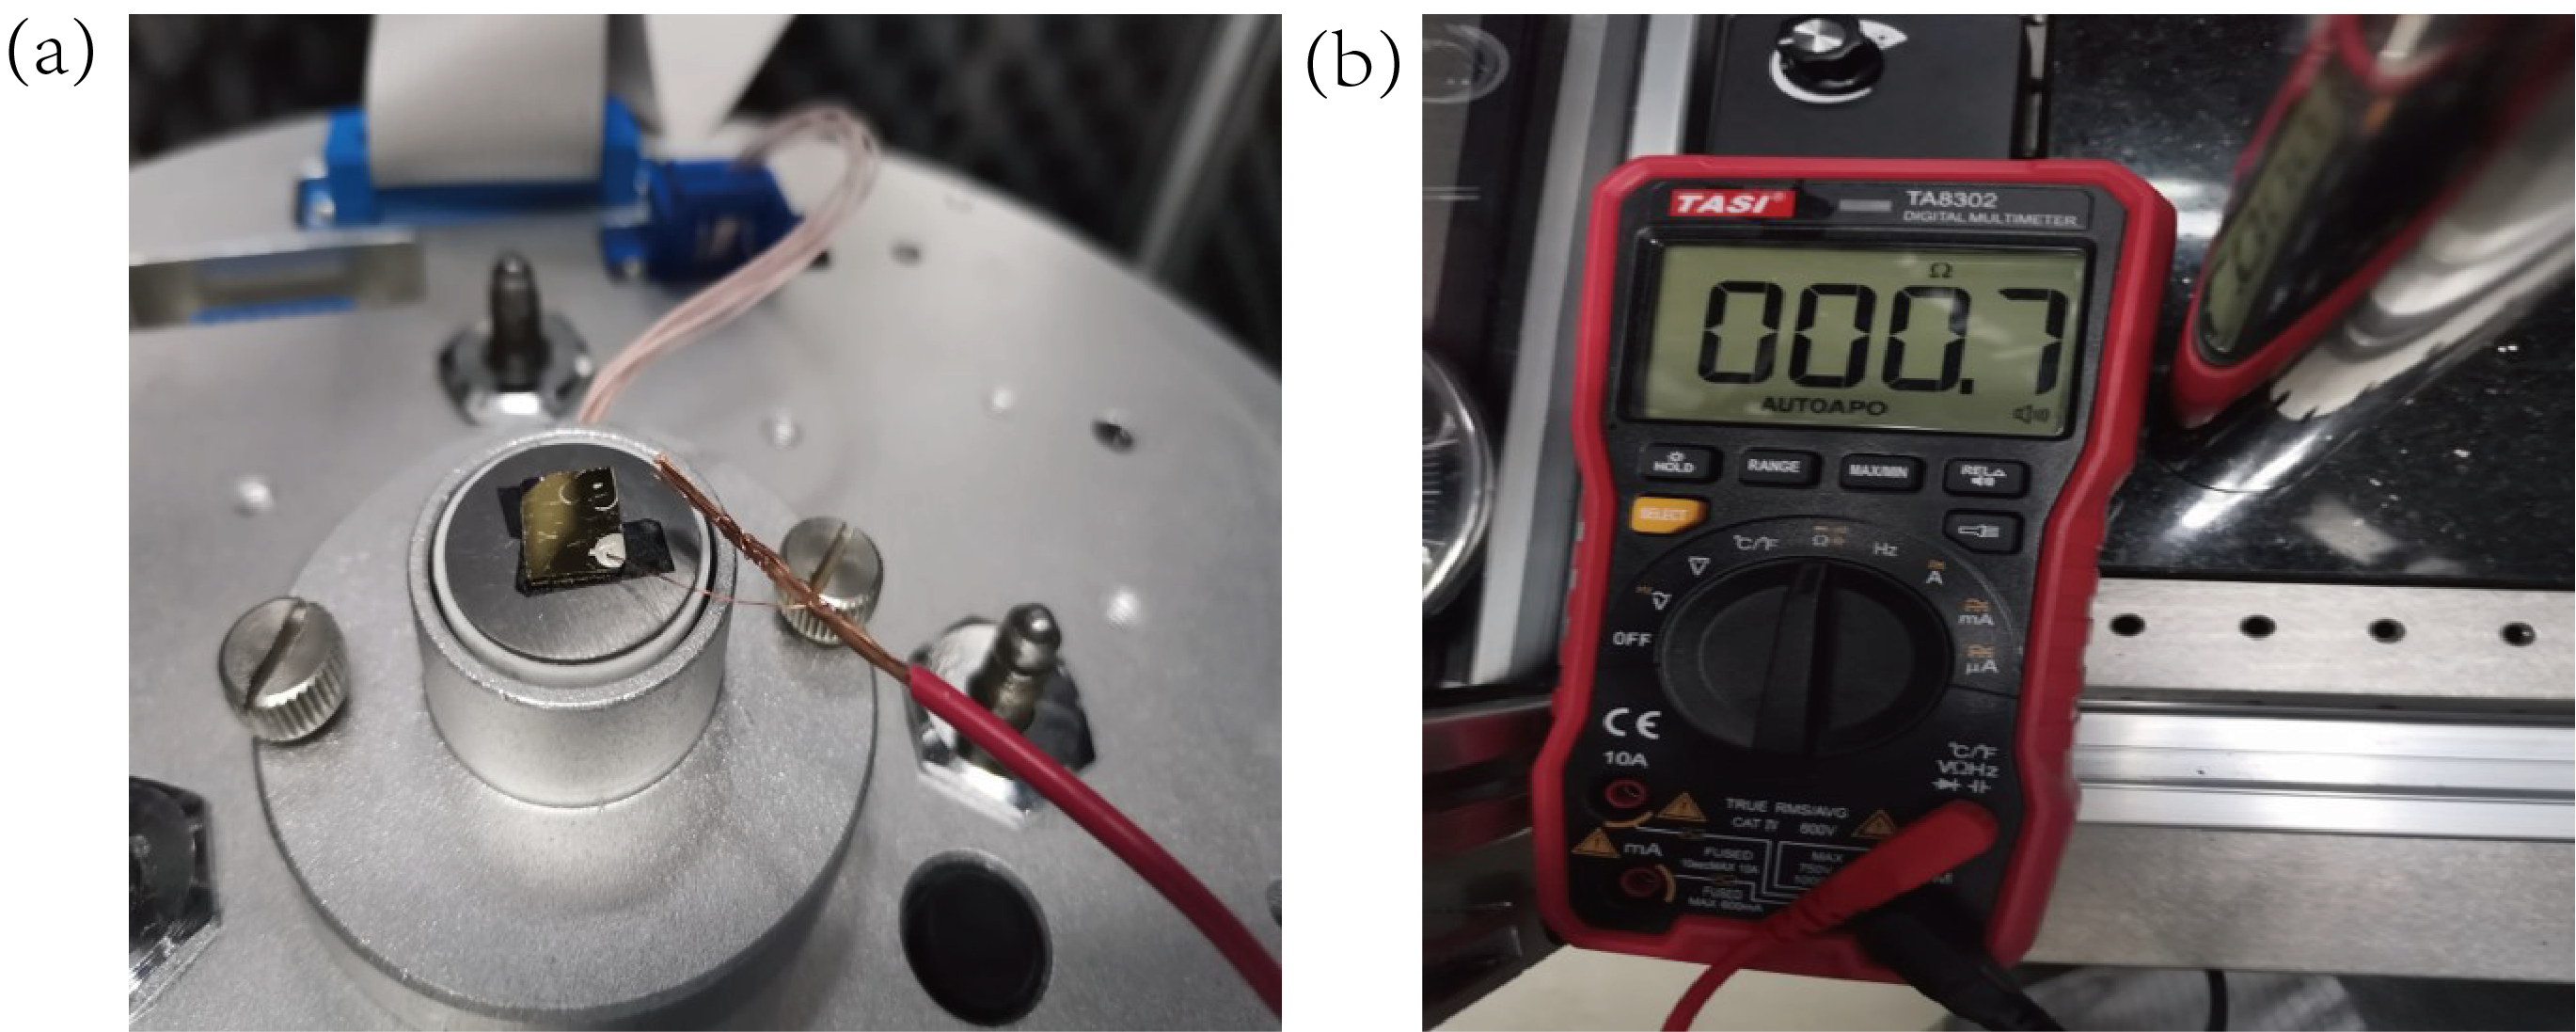
\includegraphics[scale=0.6]{figures/消除静电力}
	\caption{(a)粘上地线的样品.(b)为接地后测量的样品表面到地线之间的电阻值}
	\label{fig:10}
\end{figure}
\section{实验前的准备操作和注意事项}
\paragraph*{}
\subsection{缓冲措施}
为了减小测量过程中仪器振动带来的噪声信号,我们需要对仪器做一些减震措施,具体包括:1.为光学气垫平台充气;2.在测量过程中放下弹簧减震架。
\subsection{消除静电力的措施}
为了消除静电力的干扰,我们需要对样品接地线,同时用加湿器保持实验室湿度处于合适的范围。具体操作包括:1.在金样品表面用银胶粘上铜丝,引入地线到实验装置中,测量时将铜丝与地线缠在一起,以达到引出金样品表面电荷的目的。2.使用加湿器保持工作间湿度合适。
\subsection{正式实验前的准备操作}
在进行测量力曲线或者扫描样品的实验前,我们要将样品和探针安装在AFM装置上,并且使二者处于接触的状态。这些准备操作的具体实验步骤如下:\\
1.安装扫描管。取出S8166型扫描管,安装在扫描器上;\\
2.固定样品。用导电胶带将金样品固定在扫描管上,并连接地线和金样品上的接地线;\\
3.安装探针。取出探针架,将探针安装上去,再放回探针架。\\
4.打开控制机箱和“SPM Console”软件,选择“接触模式”。选择对应的扫描器编号并进行扫描器畸变校正。\\
5.调激光和四象限。用CCD观察激光的位置,将激光斑点调到悬臂梁上,再调节四象限,使激光斑点处于四象限的中心。\\
6.进针。选择合适的“参考点”和“积分增益”,“比例增益”值,点击软件上的“进针”按钮,直到加在压电陶瓷上的电压从180V突变为0V左右,进针结束。
\subsection{跳变距离修正}
根据哈佛大学Mariangela等人在2005年发的一篇论文\cite{Mariangela_2005},当探针和样品之间的距离很近时,悬臂梁的恢复力矩不足以克服卡西米尔力引起的外力矩,从而导致小球会突然跳变至与金板接触。跳变的距离一般在70nm左右,因此我们在数据处理时也要进行跳变距离的修正。
\section{实验设计}
\paragraph*{}
本课题的主要目的是基于Casimir效应的无接触式扫描显微镜的研究。但是在进行扫描实验之前,我们需要先测量Casimir力的性质,并且对实验装置进行改装,实现能够读出四象限的信号以及通过外加电压控制样品的移动的功能。具体的实验设计如下:
\paragraph*{}阶段一:利用仪器自带的程序测量Casimir力曲线。要想制作出基于Casimir力的无接触式显微镜,第一件要做的事就是测量出Casimir力曲线。只有测量出力曲线后我们才能根据后续实验过程中探针受的力来判断探针和样品之间的距离。
\paragraph*{}阶段二:利用外接端口读取四象限信号,并且控制扫描管的移动。我们要在扫描过程中实时地记录每个点对应的探针和样品间的距离,这是通过我们实时地读取四象限信号,将其转换为探针所受的力,然后再根据力曲线换算为探针和样品间的距离所实现的。
\paragraph*{}阶段三:对台阶样品进行无接触式扫描,研究基于Casimir效应的无接触式扫描显微镜的可行性。



\section{实验重点难点及对应的解决措施}
\paragraph*{一.采集四象限的信号}
\paragraph*{}
扫描时必须实时地采集四象限的响应信号,而系统自带的软件无法实现这个功能。
\paragraph*{}
解决措施:与厂商联系购买四象限信号的引出端口,然后使用USB-6001采集卡采集四个象限的信号并通过程序运算实现实时地采集四象限Up-Down信号的功能。
\paragraph*{}
\paragraph*{二.控制样品的移动}
\paragraph*{}
扫描时我们需要能够自行控制样品在x,y,z方向的移动,而系统自带的软件无法实现这一功能。
\paragraph*{}
解决措施:与厂商联系购买控制器“SignalIn”端口的连接线,该连接线一端连接控制器,另一端有三个接口,分别对应外加在压电陶瓷x,y,z方向上的电压。我们只要控制压电陶瓷的移动,也就能控制与之固连的样品的移动。使用USB-6001采集卡输出设定电压信号。
\paragraph*{}
\paragraph*{三.样品的倾斜摆放对实验的影响}
\paragraph*{}
即使在扫描的方向上样品倾斜的斜率只有百分之一,由于我们扫描的范围大约为100微米,在这个范围内样品的高度仍然有1000纳米的起伏,而Casimir力的力程也就大约为500纳米,因此排除样品的倾斜情况对扫描的干扰是非常有必要的。
\paragraph*{}
解决措施:首先进针使探针和样品处于接触的状态,接着在压电陶瓷z方向上加上一定大小的偏压,使样品向下运动,与针尖分离,然后沿着x方向加偏压,使样品向左移动一定距离,再缓慢减小加在压电陶瓷z方向上的电压,直到样品与探针接触,记录接触时加在压电陶瓷z方向的电压,换算成距离对应的就是在x方向上相距一定距离的两处高度差,将该高度差与水平移动的距离相除就能得到样品在x方向上的斜率。在水平扫描过程中我们就可以修改程序,根据样品的倾斜情况实时地改变加在压电陶瓷z方向上的电压,以抵消样品的倾斜对于扫描的影响。
\paragraph*{}
\paragraph*{四.静电力的干扰}
\paragraph*{}
在实验过程中,静电力会对Casimir力的探测造成很大的干扰。由于样品表面带电荷量未知,也没有办法定量地估计静电力的大小来将其在数据处理时消除。
\paragraph*{}
解决措施:用导电银胶在金样品表面粘上铜丝,从实验室外部把地线接进来,实验时将铜丝与地线缠绕在一起,达到样品接地的效果,从而引出样品表面的电荷。
\paragraph*{}
\paragraph*{五.噪声信号的干扰}
\paragraph*{}
实验过程中不可避免的会有噪声信号被引入,但是我们可以采取一些措施减小噪声信号。
\paragraph*{}
解决措施:(1)在实验前给承载原子力显微镜的气垫平台充气;(2)实验过程中放下减震弹簧。